\section{Inventory and Stock Management}

The Inventory module allows for robust tracking of stock across multiple locations, facilitating internal transfers, receipts, and deliveries.

\subsection{Inventory Overview}
Navigate to the \textbf{Inventory} app from the main dashboard. This dashboard gives a quick glance at Receipts, Deliveries, and Internal Transfers.

\begin{figure}[H]
    \centering
    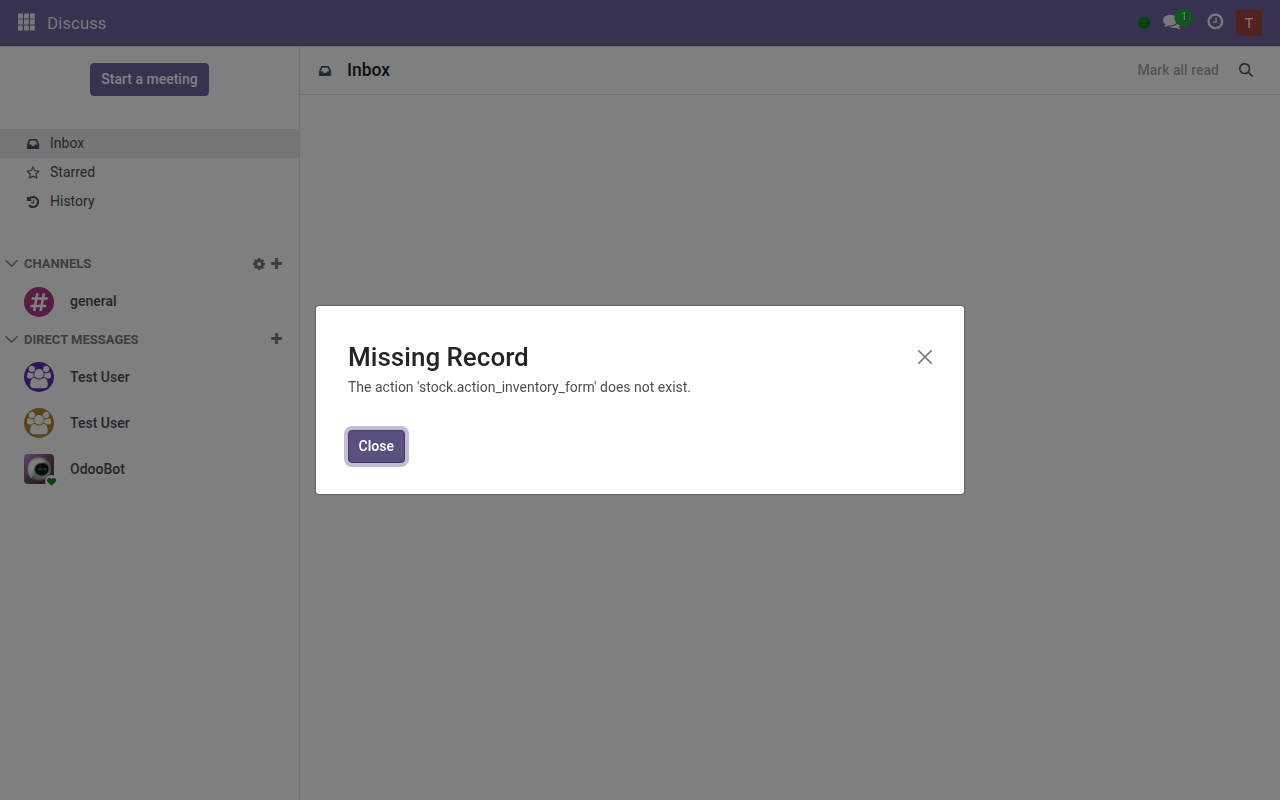
\includegraphics[width=0.9\textwidth]{images/inventory_overview.png}
    \caption{Inventory Operations Overview}
\end{figure}

\subsection{Managing Internal Transfers and Issue Notes}
An Issue Note is generated when stock is transferred internally (e.g., from a main warehouse to a manufacturing site or testing facility).

To process an internal transfer:
\begin{enumerate}
    \item Click on \textbf{Internal Transfers} from the Inventory overview.
    \item Select an existing transfer or click \textbf{New} to create one.
\end{enumerate}

\begin{figure}[H]
    \centering
    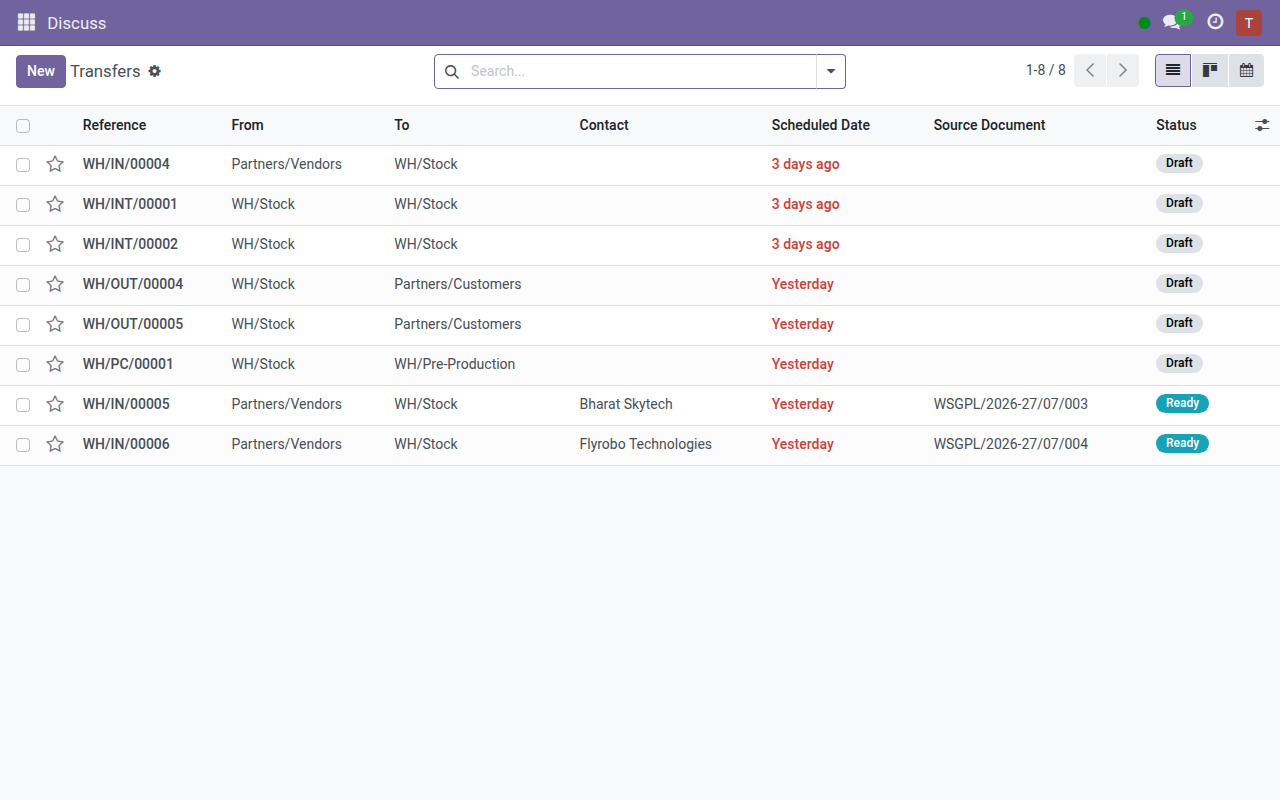
\includegraphics[width=0.9\textwidth]{images/internal_transfers_list.png}
    \caption{List of Internal Transfers}
\end{figure}

\begin{enumerate}[resume]
    \item Specify the \textbf{Source Location} and \textbf{Destination Location}.
    \item Under the \textbf{Operations} tab, add the products being transferred and set the \textbf{Demand} quantity.
    \item Click \textbf{Validate} once the products are physically moved.
\end{enumerate}

\begin{figure}[H]
    \centering
    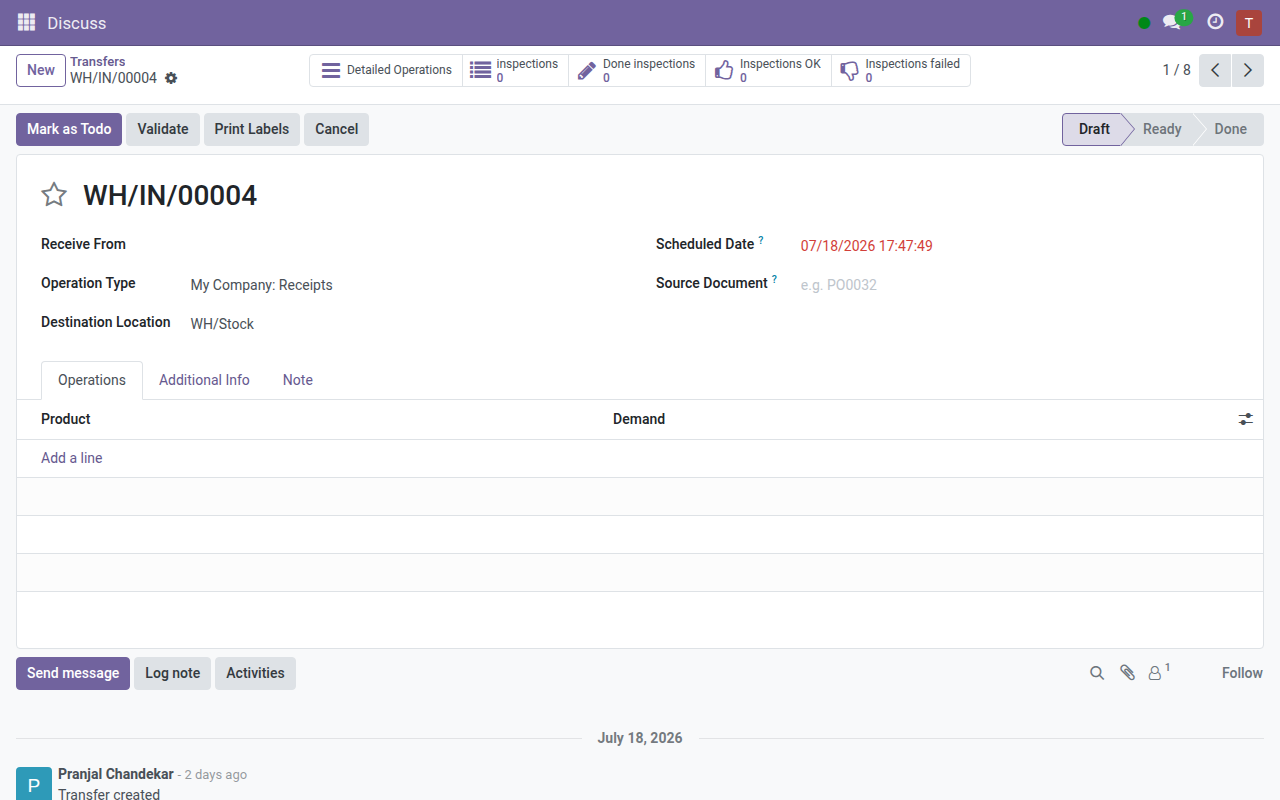
\includegraphics[width=0.9\textwidth]{images/issue_note.png}
    \caption{Detailed View of an Internal Transfer (Issue Note)}
\end{figure}

\subsection{Printing the Issue Note}
Wingspann Global requires an official Issue Note for auditing internal stock movements.
\begin{itemize}
    \item From the validated transfer screen, click the \textbf{Print} icon.
    \item Select \textbf{Issue Note}.
\end{itemize}

\begin{warnbox}
    The printed Issue Note must be signed by the \textbf{Indented By}, \textbf{Authorized By}, \textbf{Issued By}, and \textbf{Received By} personnel before the physical transfer is considered fully authorized.
\end{warnbox}

\newpage
